%\pdfoutput=1
%\documentclass[aps,pra,10pt,twocolumn,showpacs,superscriptaddress,floatfix,footinbib,subfigure]{revtex4}
\documentclass[aps,pra,12pt,onecolumn,showpacs,superscriptaddress,floatfix,footinbib,subfigure]{revtex4}

\usepackage{amsmath}
\usepackage{latexsym}
\usepackage{amssymb}
%\usepackage{bm}
\usepackage{graphicx,epstopdf,subfigure,color}
%\input{Qcircuit}
\definecolor{Red}{rgb}{1,0,0}

%braket definitions
\def\bra#1{\mathinner{\langle{#1}|}}
\def\ket#1{\mathinner{|{#1}\rangle}}
\def\braket#1{\mathinner{\langle{#1}\rangle}}
\def\ketbra#1#2{{\ket{#1}}{\bra{#2}}}
\def\Bra#1{\left\langle#1\right|}
\def\Ket#1{\left|#1\right \rangle}
{\catcode`\|=\active
  \gdef\Braket#1{\begingroup
\mathcode`\|32768\let|\BraVert\left<{#1}\right>\endgroup}}
\def\BraVert{\egroup\,\mid\,\bgroup}
\def\Brak#1#2#3{\bra{#1}#2\ket{#3}}
\def\braket#1#2{\mathinner{\langle{#1}|{#2}\rangle}}
%braket definitions
\def\es{{\mathcal{S}}}
\def\md{{\mathcal{M}}}
\def\ea{{\mathcal{A}}}
\def\sm{{\es,\md}}
\def\rs{\rho^\es}
\def\rm{\rho^\md}
\def\U{\mathcal{U}}
\def\uw{U_w^\sm}
\def\sn{ \sigma_{ \hat{n} } }
\DeclareMathOperator{\Tr}{Tr}
\DeclareMathOperator{\re}{Re}
\DeclareMathOperator{\im}{Im}
\def\sone{{\mathcal{S}_1}}
\def\stwo{{\mathcal{S}_2}}
\def\sot{{\sone\stwo}}
\def\kb#1{\ket{#1}\bra{#1}}

\newcommand{\hs}{\hspace{.5cm}}
\newcommand{\vs}{\vspace{.1cm}}

%\usepackage{cancel}
%\usepackage{color}
%\definecolor{Blue}{rgb}{0,0,1}
%\definecolor{Red}{rgb}{1,0,0}
%\definecolor{Green}{rgb}{0,1,0}
%\definecolor{Purp}{rgb}{.2,0,.2}
%\definecolor{white}{rgb}{1,1,1}




\begin{document}
\title{Experimental realization of post-selected weak measurements on an NMR quantum computer}



\begin{abstract}
 {\color{red}(We still need to add some words in abstract)}We demonstrate the first experiment of a post-selected weak measurement using a 3-qubit NMR quantum computer. Our scheme for overcoming the problem of post-selection in an ensemble quantum computer is general and can be applied to circuit-based implementation. This experiment  paves the way for studying and exploiting post-selection in systems where projective measurements are hard to realize experimentally.

\end{abstract}
\maketitle
\section{Introduction}
Most  fundamental experiments in quantum mechanics can be written in terms of a quantum circuit  \cite{Deutsch1985}. The current state of the art, however,  provides a poor platform for implanting these circuits on what can be considered a universal quantum computer. The limited number of  independent degrees of freedom  that can be manipulated efficiently limit the possible experiments. The most popular experiments with a small number of qubits are those involving non-locality and/or post-selection. Post-selection allows the {\color{red}experimentalists} condition their statistics of those experiments that (will) meet a certain criteria, usually the result of a projective measurement, at the end of the experiment. Such conditioning produces a number of surprising effects  like  strange weak values \cite{Aharonov1988} and nonlinear quantum gates \cite{Lloyd2011}. Although they are often described via quantum circuits, experiments  involving post-selection are usually implemented in a dedicated setup \textbf{which is not intended to act as a universal quantum processor} {\color{red}I am afraid guys doing optics would be unhappy with this. How about using "such as optics" and add some experimental references?}.


 {\color{red}Nowadays, implementations of quantum computing tasks in NMR architecture provide a good test-bed for up to 12 qubits  \cite{Negrevergne2006}. Besides, universal quantum circuit can nearly be achieved on the mid-scale NMR quantum computers with the development of high-fidelity control[]}. However, the difficulty in performing  projective measurements poses a  {\color{red}handicap} with the implementation of  circuits involving  post-selection. In this letter,  we will show how to overcome this  difficulty theoretically and experimentally, in the setting of weak measurements.

Weak measurements provide an elegant way to learn something about a quantum system $\es$  in the interval between preparation and post-selection. When the interaction between $\es$ and a measuring device $\md$ is weak enough, the back-action will be negligible. Moreover the effective evolution of the measuring device during the measurement is proportional to a \emph{weak value}, a complex number which is a function of the pre-selection, post-selection and the desired observable. These weak values allow us to make statement that would otherwise be in the realm of \emph{counterfactuals}. Weak values have been interpreted  as complex probabilities \cite{Hofmann2013} and/or  \emph{element of reality} \cite{Vaidman1996} and, although somewhat controversial \cite{Peres1989, Aharonov1989, Leggett1989}, they are  used to explain a number of fundamental issues in quantum mechanics including: Non-locality in the two slit experiment[ ], the reality of the wave function[ ], Hardy's paradox[ ], the three box paradox [ ]and  measurement precision-disturbance relations[]; they are also used for violating the Leggett-Garg inequality \cite{Goggin2011,Williams2008}. Recently weak measurements were also found to be useful as a practical tool for precision measurements due to the  amplification effect of weak values with a large real or imaginary part.  While these schemes cannot overcome the limits imposed by quantum mechanics, they can be used to improve precision under  various types of operational imitations  such as \emph{technical noise} [].

Weak measurement experiments have so far been limited to the realm of optics with a few (very recent)  deviations \cite{Shomroni2013, Groen2013} . In most cases the experiments exploited the fact that one degree of freedom can be used as the system while another (usually a continuous parameter) can be used as the measuring device.  Post-selection is usually done by filtering out photons that fail post selection and the readout is done at the end only on the surviving systems. This type of filtering is outside the scope of ensemble quantum computers where all operations apart from the final ensemble measurement are unitary. One can overcome the difficulty by either adding including a filtering operation or by finding some way for post-selection using unitary operations. The former poses a technical challenge  as well as a conceptual deviation from the circuit model. In what follows we show how to perform the latter by resetting the measuring device each time post-selection fails.

 We begin by describing the weak measurement process for qubits and the theoretical circuit  for weak measurements on an ensemble quantum computer. Next we describe our experiment in detail. We conclude with a discussion of future applications.

%===========================================================================================================================================

\section{Weak measurements}
The weak measurement  procedure (for qubits) \cite{Brun2008}  involves a system $\es$ qubit  initially prepared in the state $\ket{\psi}^\es$ and a measuring device qubit  initially in the state $\ket{\md_i}^\md$. The system and measuring device are coupled for a very short time  via the interaction  Hamiltonian  $H_i=\delta(t-t_i)g\sn^\es\sigma_z^\md$ with $g<<1$ the coupling constant and $\sn=\hat{n}\cdot\vec{\sigma}$ a Pauli observable in the direction $\hat{n}$.  This is followed by a projective (post-selection) measurement on $\es$ with outcome $\ket{\phi}^\es$. So, up to normalization we have

\begin{equation}
\ket{\psi,\md_i}^\sm\rightarrow e^{-g\sn^\es\sigma_z^\md}\ket{\psi,\md_i}^\sm \rightarrow \cos(g)\langle {\phi}|{\psi}\rangle \ket{\phi,\md_i}^\sm+i\sin(g)\bra{\phi}\sn\ket{\psi}\sigma_z^\md\ket{\phi,\md_i}^\sm
\end{equation}

The unnormalized state of $\md$ at the end is
\begin{equation}
\ket{\md_f}=\langle {\phi}|{\psi}\rangle[ \cos(g)\openone^\md+i\sin(g)\{\sn\}_w\sigma_z^\md]\ket{\md_i}^\sm
\end{equation}

where $\{\sn\}_w=\frac{\bra{\phi}\sn^\es\ket{\psi}}{\langle {\phi}|{\psi}\rangle}$ is the weak value of $\sn$. We can now take the weak measurement approximation $|\sin(g)\{\sn\}_w|<<\cos(g)$ so that up to first order in $g$ we have
\begin{equation}
\ket{\md_f}\approx e^{ig\{\sn\}_w\sigma_z}\ket{\md_i}
\end{equation}

The measurement device is rotated by $g\{\sigma_z\}_w$ around the $z$-axis.  Note that this is the actual unitary evolution (at this approximation), not an average unitary.  If we set the measuring device to be in the initial state $\frac{1}{\sqrt{2}}[\ket{0}+\ket{1}]$,  the  expectation value for $\sigma_m^\md=\hat{m}\cdot\vec{\sigma}^\md$ will be
\begin{align}\label{readout}
\bra{\md_f}\sigma_m^\md\ket{\md_f}&=\bra{\md_i}(\openone+ig\{\sigma_z\}_w^*\sn^\md)\sigma_n^\md(\openone-ig\{\sn\}_w\sigma_z^\md)\ket{\md_i}\\&\approx\bra{\md_i}\sigma_m^\md\ket{\md_i}+ig\bra{\md_i}\{\sn\}_w^*\sigma_m^\md\sigma_z^\md-\{\sigma_z\}_w\sigma_z^\md\sigma_m^\md\ket{\md_i}\\
\label{ReIm}&=\bra{\md_i}\sigma_m^\md\ket{\md_i}\\&\;+ig\bra{\md_i}Re(\{\sn\}_w)[\sigma_z^\md,\sigma_m^\md]-iIm(\{\sn\}_w)\{\sigma_z^\md,\sigma_m^\md\}\ket{\md_f}\nonumber
\end{align}
Choosing $\hat{n}$ appropriately we can get either the real or imaginary part of the weak value.

The scheme above is based on the fact that $\es$ was post-selected in the correct state $\ket{\phi}$. Since this cannot be guaranteed in an experiment we need to somehow disregard those events when post-selection fails.  As noted previously the standard method for implementing the post-selection is by filtering out the composite $\sm$ systems that fail post-selection. While this is relatively simple in some optical implementations it  cannot be done on a generic quantum processor. The method to overcome this problem (see Fig. \ref{circuit}) is to reset the measuring device whenever post-selection fails. This can be  done using a controlled depolarizing gate with the following properties
\begin{align}\label{Cdepol}
\ket{\phi}\bra{\phi}^\es\otimes\rho^\md&\rightarrow \ket{\phi}\bra{\phi}^\es\otimes\rho^\md \nonumber\\
\kb{\phi^\perp}^\es\otimes\rho^\md &\rightarrow \kb{\phi^\perp}^\es\otimes\openone/2,
\end{align}
where  $\rho^\md$ is an arbitrary state and $\ket{\phi^\perp}^\es$ is the orthogonal state to the post-selection  $\bra{\phi^\perp}\ket{\phi}=0$.

This gate is not unitary and requires an ancillary system $\ea$. It can be  constructed (see Fig. \ref{circuit}) by setting $\rho^\ea=\openone/2$ and using a controlled-SWAP with the swap between $\ea$ and $\md$. To keep the control in the computational basis, we  preceded the controlled-SWAP gate by $U_\phi^{\es\dagger}$ where $U_\phi\ket{0}=\ket{\phi}$.  At the readout stage we now need to measure the observable $\kb{0}$ which will give the probability of post-selection $p_0$. Finally we divide the readout on $\md$, Eq. \eqref{readout}, {\color{red} what does eq 4 mean here?} by $p_0$ to obtain the desired weak value. If we are  only interested in obtaining the weak value, we can further simplify this operation by a controlled dephasing in the a complementary basis to the readout. This allows us to replace the controlled-SWAP by a controlled-controlled-phase with $\md$ as the target and $\ea,\es$ as the control (see Fig. \ref{molecule}(b).).


\begin{figure}[h] \centering

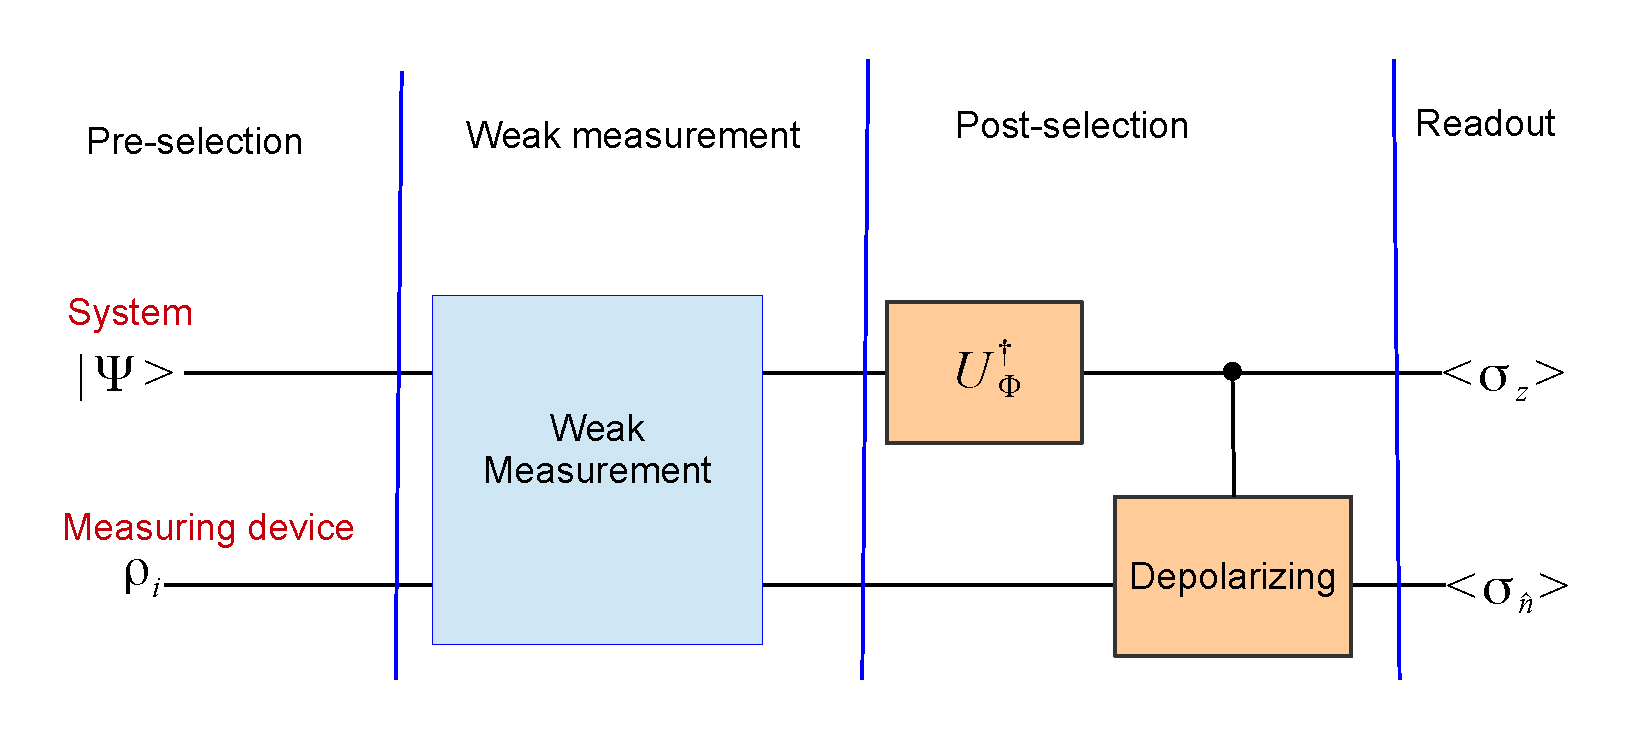
\includegraphics[width=\columnwidth]{Theory.pdf}
\caption{The general circuit for a post selected weak measurement. The system is prepared in the state $\ket{\psi}$, it then interacts weakly with the measurement device (the weak measurement stage). Post selection is performed by a controlled depolarizing channel in the desired basis, Eq \eqref{Cdepol}, decomposed into a rotation $U^\dagger_\phi$ followed by a contolled depolarizing in the computational basis. Finally at the readout stage we get the probability of post-selection with  $<\sigma_z^\es>=2p_0-1$ and the exception values on $\md$  shifted by a factor proportional to the weak value and decayed by a factor $1-p_0$. }\label{circuit}
\end{figure}

%=========================================================================================================================
\section{Experimental Implementation}
For the experimental implementation, we use $^{13}$C labeled trichloroethylene (TCE) dissolved in d-chloroform as a 3-qubit sample. All experiments were conducted on a Bruker DRX 700MHZ spectrometer at room temperature. The structure of the molecule is shown in Fig. \ref{molecule}(a), where we denote C1 as qubit 1, C2 as qubit 2, and H as qubit 3. The internal Hamiltonian of this system can be described as
\begin{eqnarray}\label{Hamiltonian}
\mathcal{H}=&&\sum\limits_{j=1}^3 {\pi \nu _j } \sigma _z^j  + \frac{\pi}{2}(J_{13}\sigma _z^1 \sigma _z^3+J_{23}\sigma _z^2 \sigma _z^3) \nonumber\\
&&+ \frac{\pi}{2}J_{12} (\sigma _x^1 \sigma _x^2+\sigma _y^1 \sigma _y^2+\sigma _z^1 \sigma _z^2),
\end{eqnarray}
where $\nu_j$ is the chemical shift of the $j$th spin and $J_{ij}$ is the scalar coupling strength between spins $i$ and $j$. As the difference in frequencies between C1 and C2 is not large enough to adopt the (NMR \footnote{We distinguish the term weak coupling as used in NMR from the term weak interaction used for the weak measurement}) weak J-coupling  approximation \cite{nmrreview}, these two carbon spins are treated in the strongly coupled regime. The parameters of the Hamiltonian are obtained by iteratively fitting the calculated and observed spectra through perturbation, and shown in the table of Fig. \ref{molecule}(a).

\begin{figure}[h] \centering
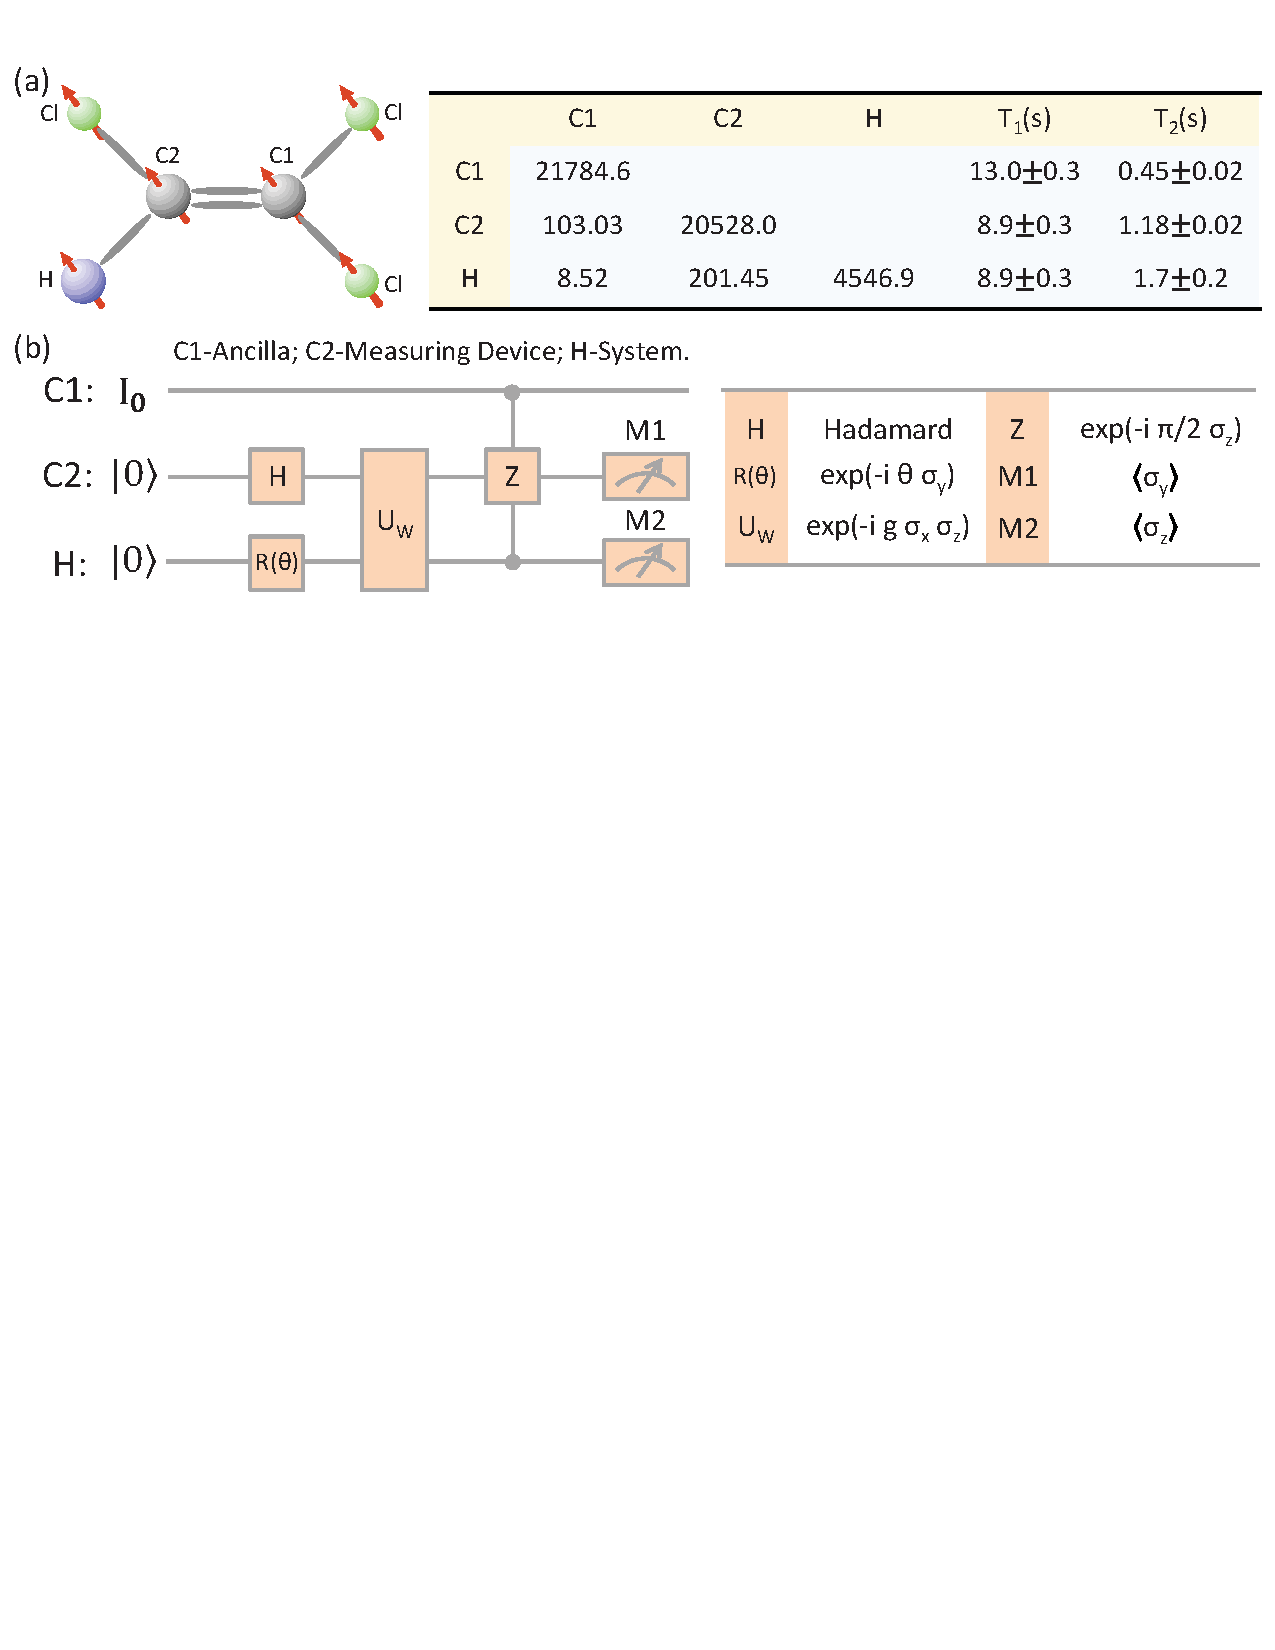
\includegraphics[width=\columnwidth]{molecule.pdf}
\caption{(color online). (a) Molecular structure of trichloroethylene in which the two $^{13}$C and one $^{1}$H spins form a 3-qubit sample, and the system parameters. In the parameter table, the diagonal elements are the chemical shifts (Hz), and the off-diagonal elements are scalar coupling strengths (Hz). The relaxation and dephasing time scales T$_1$ and T$_2$ are also listed in the table. (b) Quantum network to realize the post-selected weak measurement in experiment. Here, C1 is used as the ancilla, C2 as the measuring device, and H as the system. }\label{molecule}
\end{figure}

 To realize the post-selected weak measurement, we label C1 as the ancilla, C2 as the measuring device, and H as the system displayed in Fig. \ref{molecule}(b). After the labeling, the experiment can be divided into four parts: (A) Pre-selection. We initialize the ancilla to the identity matrix $I$, the measurement device to $1/\sqrt{2}(|0\rangle+|1\rangle) $, and the system to $cos\theta|0\rangle+sin\theta|1\rangle$. (B) Weak measurement through the interaction between the measuring device and system, denoted by U$_w$ in the network. (C) Post-selection of the system in the state $|0\rangle$. (D) Measurement of $\langle \sigma_y \rangle$ on the measuring device and $\langle \sigma_z \rangle$ on the system. The experimental details of the four  parts above are as follows.

 (A) Pre-selection:  Starting from the thermal equilibrium state, first we excite the ancilla C1 to the transverse field by a $\pi/2$ rotation, followed with a gradient pulse to destroy the coherence. Thus the state of C1 will be maximally mixed state $I$. Secondly we create the pseudopure state (PPS) of the measuring device C2 and system H with deviation $I \otimes \kb{00}$ using the spatial average technique \cite{spatial}. The spectra of the PPS followed by $\pi/2$ readout pulses are shown in the upper part of Fig. \ref{gweak}(a). The readout pulses are applied on C2 (left figure) and H (right figure), respectively. Two peaks are generated in the PPS spectra because C1 is in the maximally mixed state $I$, and these two peaks are utilized as the benchmark for the following experiments. Thirdly we apply one Hadamard gate on C2 and one $R_y(\theta) = e^{-i\theta\sigma_y}$ rotation on H. Therefore, we have prepared the initial state for the experiment
 \begin{eqnarray}\label{pps}
 \rho_{ini}= &&I\otimes \frac{1}{2} (|0\rangle + |1\rangle) (\langle 0 | + \langle 1 |) \nonumber\\
 &&\otimes  (cos\theta|0\rangle + sin\theta|1\rangle)(cos\theta\langle 0 | + sin\theta\langle 1 |),
 \end{eqnarray}
 and finished the pre-selection step.

 (B) Weak measurement. The unitary operator to realize the weak measurement is
 \begin{equation}\label{uw}
U_w=e^{-ig\sigma_x^2 \sigma_z^3}.
 \end{equation}
 Without loss of generality, we have chosen the observable of the measuring device as $\sigma_x$. $U_w$ can be simulated by the interaction term $\sigma_z^2\sigma_z^3$ between C2 and H using the average Hamiltonian theory \cite{ernstbook}. However, since the internal Hamiltonian contains strongly coupling term and the refocusing scheme requires the complicated WAHUHA-4 sequence \cite{wahuha}, we have adopted the gradient ascent pulse engineering (GRAPE) technique \cite{grape1,grape2} to improve the fidelity. We will discuss it in detail later in this letter.

 (C) Post-selection. In order to mimic the post-selection of $|0\rangle$ on the system spin H in NMR, we introduce an ancilla qubit C1 in the maximally mixed state $I$. The controlled resetting noise operation is thus a controlled-controlled-$\sigma_z$ gate
 \begin{equation}\label{postselection}
I\otimes I \otimes I - |1\rangle \langle 1 | \otimes I \otimes  |1\rangle \langle 1 | + |1\rangle \langle 1 | \otimes |1\rangle \langle 1 | \otimes \sigma_z.
 \end{equation}
 If post-selection is successful, the measurement device will point to the weak value. Otherwise the measurement device will become dephased.

(D) Measurement. Finally we measure the expectation value $\langle \sigma_y^2 \rangle$ on C2 and $\langle \sigma_z^3 \rangle$ on H, to calculate the weak value by the expression
 \begin{equation}\label{weakvalue}
\{ \sigma_x \}_w \approx \frac{\langle \sigma_y^2 \rangle}{ g(\langle \sigma_z^3 \rangle+1)}.
 \end{equation}

In the experiment, the $\pi/2$ rotation of H is realized by the hard pulse with a duration of 10 $\mu$s. All the other operations are packed into GRAPE pulses to achieve high-fidelity control. These GRAPE pulses are designed to be robust to the inhomogeneity of the magnetic field, and the imprecisions of the parameters in the Hamiltonian. For the two selective $\pi/2$ excitations on C1 and C2, the GRAPE pulses are generated with the length 1.5 ms, segments 300 and fidelity over 99.95\%. These two pulses are only used for the preparation and observation of PPS. Besides these two GRAPE pulses, the PPS preparation involves another GRAPE pulse of 10 ms and 99.99\% fidelity for the creation of two-body coherence. The upper part of Fig. \ref{gweak}(a) shows the spectra of the PPS both on C2 and H, which are used as the benchmark for the following experiments.

The main body of the network shown in Fig. \ref{molecule}(b), including the pre-selection, weak measurement and post-selection, is calculated by a single GRAPE pulse. Since we have to alter the initial state by $\theta$ and interaction strength $g$ in the experiment, we have used different GRAPE pulses to implement the experiments with different group of parameters. All of these GRAPE pulses have the same length 20 ms, and fidelity over 99.98\%.

There are two essential advantages in utilizing the GRAPE pulses: reducing the error accumulated by the long pulse sequence if we directly decompose the network, and reducing the error cause by the decoherence. Because the $U_w$ evolution is supposed to be very "weak", the intensity of the output signal is quite small. Moreover, the weak value $\{ \sigma_x \}_w$ is more sensitive to the intensity of the signal, because the small $g$ existing in the denominator (Eq. \ref{weakvalue}) will amplify the errors in the experiment. Therefore, we need to achieve as accurate coherent control as we can to obtain precise experimental results. The direct decomposition of the original network requires many single rotations, as well as a relatively long evolution time. For example, an efficient way to decompose the controlled-controlled-$\sigma_z$ gate is by six CNOT gates and several one qubit gates \cite{chuangbook}, which requires more than 50 ms in our experimental condition. Therefore, using \emph{short} GRAPE pulses of \emph{high fidelity} is able to decrease the potential errors extremely in these experiments. The lower part of Fig. \ref{gweak}(a) gives the experimental spectra compared with the simulated one in the case $g=0.05$ and $\theta = 1.4$. The predicted value of $\langle \sigma_y^2 \rangle$ in this case is only 1.67\%. However, since the experimental spectra match very well with the simulated one, we can obtain a good result after extracting the data. See Fig \ref{gweak}(b).

In experiment, firstly we choose three different groups of pre-selected state: $\theta = 1.4$, $\theta = 1.2$, and $\theta =\pi/4$. Then we vary the interaction strength $g$ between the measuring device and system from $g=0.05$ to $g = 0.7$ for a definite $\theta$, and measure $\langle \sigma_y^2 \rangle$ on the measuring device C2 and $\langle \sigma_z^3 \rangle$ on the system H, respectively. The weak value $\{ \sigma_x \}_w$ can be calculated through Eq. \ref{weakvalue}, with the result shown in Fig. \ref{gweak}(b). The error bars are obtained by repeating the experiment for four times and so forth. The large error bars in the weak values when $g$ is small can be contributed to the minor imperfect calibrations of the low experimental signals, and the loss of weak values is mainly caused by the decoherence effect. With the $g$ growing bigger, we can obviously see the experimental data become much better, as the weak measurement is getting closer to strong measurement.

\begin{figure}[h] \centering
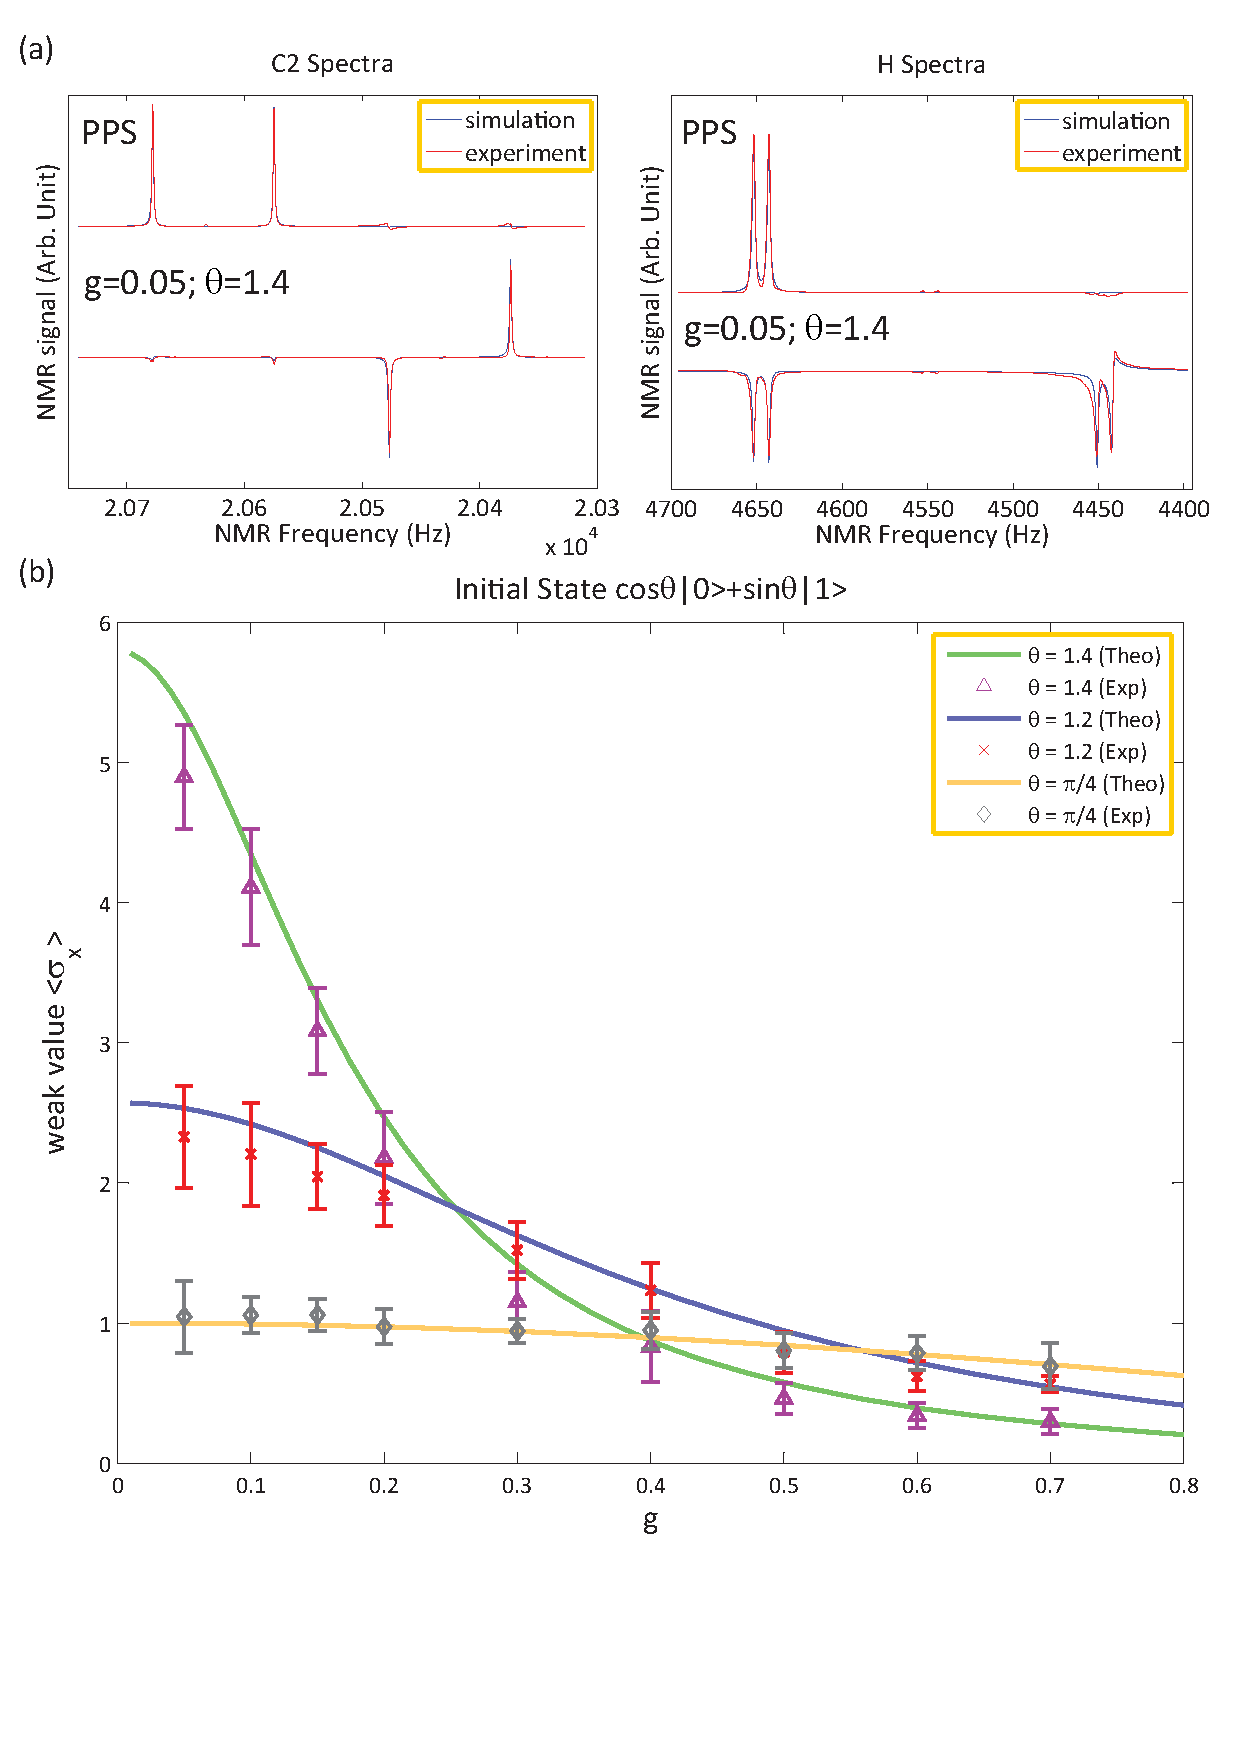
\includegraphics[width=\columnwidth]{gweak.pdf}
\caption{(color online). (a) Spectra for observing $\langle \sigma_y^2 \rangle$ on C2 and $\langle \sigma_z^3 \rangle$ on H in the case $g=0.05$ and $\theta = 1.4$ (lower part), comparing with the PPS spectra (upper part). The blue one is the simulated spectra, while the red one is the experimental spectra. To observe the signal of PPS and $\langle \sigma_z^3 \rangle$ on H, we have applied $\pi/2$ readout pulses after the sequence. To observe the signal of $\langle \sigma_y^2 \rangle$ on C2, we do not need to apply any readout pulses. (b) Experimental result for $g$ $vs$ weak values at three different  initial states. The error bars are plotted by repeating four times experiments.}\label{gweak}
\end{figure}

Secondly we observe the behavior of $\theta$ $vs$ weak by setting $g=0.1$. The theory predicts it should be a perfect $tan\theta$ function when the interaction is infinity weak, $i.e.$, $g$ is infinity close to 0. However, our simulation for $g=0.1$ shows there is singularity when $\theta$ approaches to $\pi/2$ (Fig. \ref{thetaweak}(a)). The explanation is when $\theta$ approaches to $\pi/2$, the approximation of the Taylor expansion for small $g$ will be no longer valid. In other words, $g=0.1$ is not small enough to catch up with the effect of $\theta \rightarrow \pi/2$. The experimental data, to some extent, match with the smooth part of the curve. When $\theta$ is very close to  $\pi/2$, we are not able to measure the extremely low NMR signals in this situation due to the signal-to-noise ratio(SNR) issues.

\begin{figure}[h] \centering
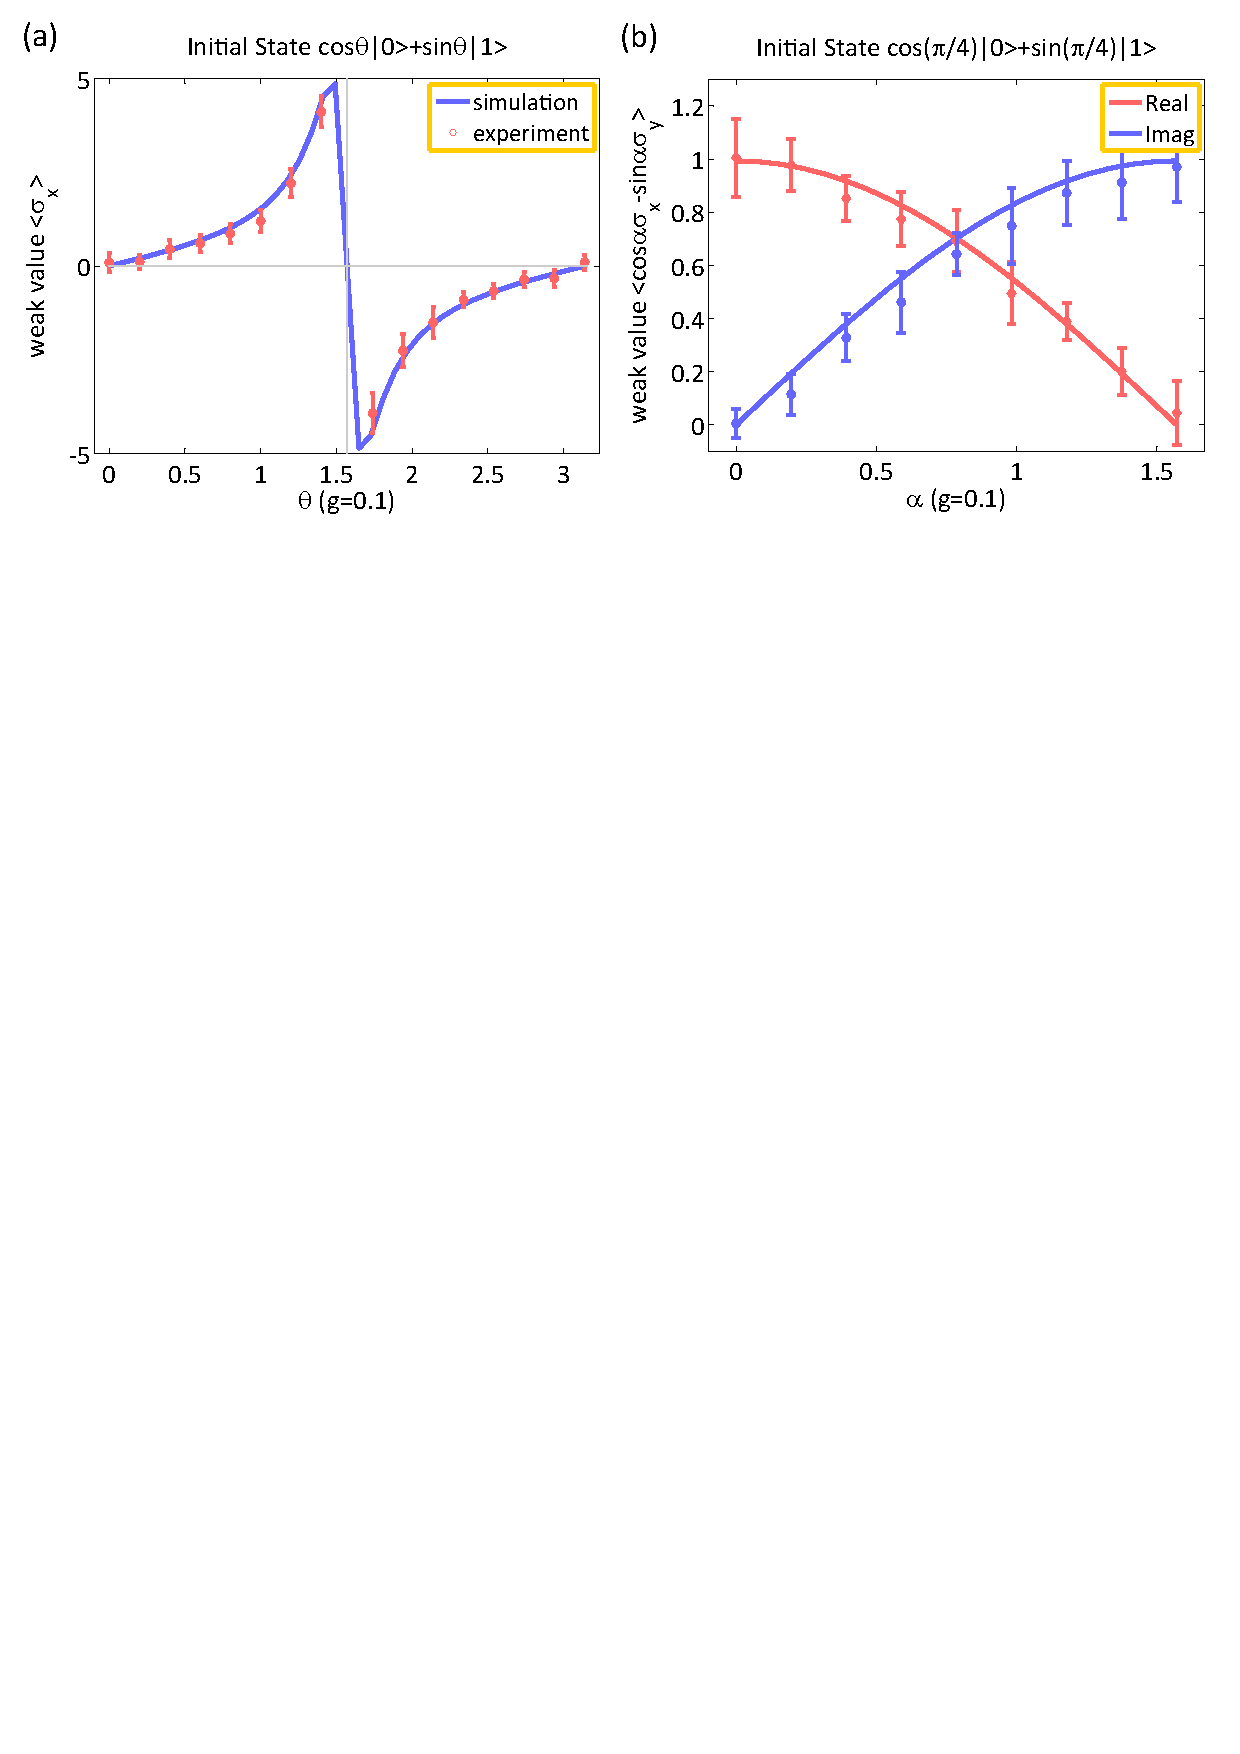
\includegraphics[width=\columnwidth]{thetaweak.pdf}
\caption{(color online). (a) Experimental result of the weak values by changing $\theta$ at $g=0.1$. The simulated (blue) curve is plotted by assuming the weak measurement approximation, and the experimental data are denoted by red circles. (b) Experimental result of measuring both the real and imaginary parts of the weak value at $g=0.1$ and $\theta = \pi/4$. Here we change the observable of the measuring device C2 to $cos\alpha \sigma_x - sin\alpha \sigma_y$.}\label{thetaweak}
\end{figure}

Finally we measure both the real part and imaginary part of the weak value (Fig. \ref{thetaweak}(b)). Here we set $\theta = \pi/4$ and $g=0.1$, and change the observable of the measuring device C2 in the $x-y$ plane by
 \begin{equation}\label{imag}
cos\alpha \sigma_x - sin\alpha \sigma_y.
 \end{equation}
 It is easy to know that the real part of the weak value becomes smaller while the imaginary part of the weak value becomes larger with $\alpha$ varying from 0 to $\pi/2$. To measure the imaginary part, we replace the controlled-controlled-$\sigma_z$ gate in Fig. \ref{molecule}(b) with a controlled-controlled-$\sigma_x$ gate, and measure the expectation value $<\sigma_z^2>$ on the measuring device C2. The other parts of the experiments remain the same. From Fig. \ref{molecule}(b), we can see the alternations of the real part and imaginary part of the weak value along with the parameter $\alpha$.
%\begin{equation}\label{pps}
 %\rho_{I00}=(1-\epsilon)\mathbb{{I}}/8+\epsilon I_0/2 \otimes | 00 \rangle \langle 00 |
 %\end{equation}
 %The thermal equilibrium state in NMR can be written as $\rho_{th} = \sum\nolimits_{i=1}^{3} {\gamma_i \sigma_z^i}$, where $\gamma_i$ is the gyromagnetic ratio for different species of nuclear spins. Typically, $\gamma$_C $=1$ and $\gamma$_H $=4$.

\section{Conclusions and outlook}
Post-selection is a useful and interesting conceptual and practical tool. Its experimental implementation have so far  been limited to {\color{red}some dedicated quantum devices}. Here we showed that this paradigm can be realized in a more general setting of a quantum circuit with unitary gates. Our experiment involved a simple 3-qubit system and we were able to demonstrate the measurement of large and imaginary weak values. Both are artifacts of post-selection. Our experimental setup allowed us to accurately measure a weak value of $2.33$ with an accuracy of $\pm0.36$ at $g=0.05, \theta=1.2$. The largest relative shift observed was  $4.90\pm  0.37$ at   $g=0.05$ and $\theta=1.4$. However, the interaction strength was too large to reach the theoretical  weak value of $5.8$.  For complex weak values we were able to demonstrate  the full spectrum of complex weak values with unit  absolute magnitude.

Our scheme has the advantage that it can be extended to systems with more qubits without significant changes.  Implementations on a four qubit system will allow (the first?) fully quantum  implementation of the three box paradox  and further extensions will allow more intricate experiments such as the measurement of the wave-function,  measurement-disturbance relations which have so far been limited to optical implementations, often with classical light. The reasonably large amount of qubits  that can be manipulated   in NMR systems will also allow more intricate experiments which are not possible in optics.  It remains an open question whether our techniques can be used for precision measurements in the same way as they are used in optics.  Given that this is the first implementation there is still much to be explored.





\section{References}
\bibliography{C:/users/abrodutch/Dropbox/fullbib}

\end{document} 